\documentclass[aspectratio=169,11pt]{beamer}
\usepackage[T1]{fontenc}
\usepackage[utf8]{inputenc}
\usepackage{lmodern,amsmath,amssymb,graphicx,tikz}
\usetikzlibrary{arrows.meta,calc}
\usetheme{default}
\usefonttheme{serif}
\setbeamercolor{normal text}{fg=black,bg=white}
\setbeamercolor{structure}{fg=black}
\setbeamercolor{frametitle}{fg=black}
\setbeamercolor{title}{fg=black}
\setbeamertemplate{navigation symbols}{}
\setbeamertemplate{footline}[frame number]
\setbeamertemplate{itemize items}[circle]
\setbeamersize{text margin left=8mm,text margin right=8mm}
\setlength{\parskip}{5pt}
\newcommand{\cO}{\mathcal O}
\newcommand{\cI}{\mathcal I}
\newcommand{\cA}{\mathcal A}
\newcommand{\db}{\bar\partial}
\newcommand{\C}{\mathbb C}
\newcommand{\Pj}{\mathbb P}
\newcommand{\norm}[1]{\lVert#1\rVert}
\newcommand{\src}[1]{\par\vfill{\scriptsize #1\par}}
\author{Daniel Gonz\'alez Casanova Azuela}

\title{Kodaira embedding theorem (Part 1)}
\subtitle{Lecture 23: the mechanism and Nadel's theorem}
\date{Hodge theory}
\begin{document}
\begin{frame}\titlepage\end{frame}
\begin{frame}{The course so far}
\begin{enumerate}
\setlength{\itemsep}{12pt}
\item \textbf{Complex structures and holomorphic functions.}\\
\(I^2=-1\), Cauchy's formula, and complex manifolds.
\item \textbf{Integrability.}\\
Frobenius, real analytic methods, and Newlander--Nirenberg.
\item \textbf{Kähler geometry.}\\
Homogeneous examples and Fubini--Study; Levi-Civita, intrinsic torsion, and Bismut.
\end{enumerate}
\end{frame}

\begin{frame}{The course so far (continued)}
\begin{enumerate}
\setcounter{enumi}{3}
\setlength{\itemsep}{9pt}
\item \textbf{Hodge theory and Kähler identities:} harmonic representatives.
\item \textbf{Sheaves and Dolbeault:} cohomology through the \(\db\)-complex.
\item \textbf{Chern curvature and bundle-valued Hodge theory:}\\
Bochner--Kodaira and Kodaira--Nakano vanishing.
\item \textbf{The analytic extension:} Hilbert-space operators and \(L^2\);
holomorphic convexity, Stein spaces, and pseudoconvex vanishing;
currents, singular psh weights, and Poincaré--Lelong.
\end{enumerate}
\end{frame}

\begin{frame}{Reminder: curvature and positivity}
Every Hermitian holomorphic line bundle \((L,h)\) has a unique \textbf{Chern connection} \(\nabla\): it preserves \(h\) and its \((0,1)\)-part is \(\db_L\).
\par\medskip
Its square is multiplication by a two-form, the \textbf{curvature}:
\[
\nabla^2=\Theta_h\wedge,\qquad c_1(L)_{\mathbb R}=\left[\frac{i}{2\pi}\Theta_h\right].
\]
\(i\Theta_h\) is a real closed \((1,1)\)-form.
\par\medskip
A real \((1,1)\)-form \(\alpha\) is \textbf{positive} if \(\alpha(v,Iv)>0\) for every tangent vector \(v\ne0\).
\par\smallskip
\(L\) is \textbf{positive} if it has a smooth metric with \(i\Theta_h>0\).
\end{frame}

\begin{frame}{Projective space has a positive form}
A point of \(\Pj^n\) is a line through the origin in \(\C^{n+1}\). The map \(\pi\colon\C^{n+1}\setminus\{0\}\to\Pj^n\) sends each nonzero vector to the line it spans.
\par\medskip
On nonzero vectors \(Z\in\C^{n+1}\), define
\[
\tilde\omega=\frac{i}{2\pi}\,\partial\db\log|Z|^2,\qquad |Z|^2=|Z_0|^2+\cdots+|Z_n|^2.
\]
It is \textbf{basic}: for every vector field \(V\) along the fibres of \(\pi\),
\[
\iota_V\tilde\omega=0,\qquad \mathcal L_V\tilde\omega=0.
\]
So it comes from a form downstairs, the \textbf{Fubini--Study form}: \(\tilde\omega=\pi^*\omega_{\rm FS}\).
\par\medskip
\(\omega_{\rm FS}\) is \textbf{positive}: it gives every nonzero tangent vector a positive squared length.
\src{Basic forms: H.~Bursztyn, \emph{Geometria Simpl\'etica} (IMPA 2024), \href{https://github.com/danimalabares/sg/blob/main/listas/q3.pdf}{\textcolor{blue}{\underline{Lista 3}}}, Problem 5; M.~Verbitsky, \emph{Complex surfaces} (IMPA 2025), \href{http://verbit.ru/IMPA/Surfaces-2025/assign-surfaces-2025-04.pdf}{\textcolor{blue}{\underline{home assignment 4}}}, Exercises 4.5--4.7.}
\end{frame}

\begin{frame}{Why \(\omega_{\rm FS}\) is positive: the potential \(\ell\)}
\label{fr:fs-positive}
\textbf{Notation.} \(\ell=|Z|^2=\sum_j Z_j\bar Z_j\) and \(d^c=\frac{i}{2}(\db-\partial)\), so that \(dd^c=i\partial\db\). So \(\tilde\omega=\frac{1}{2\pi}\,dd^c\log\ell\).
\par\smallskip
\textbf{Squared length} of \(v\) means \(\alpha(v,Iv)\). Positive means: \(\alpha(v,Iv)>0\) for \(v\ne0\).
\begin{enumerate}
\item \textbf{Differentiate.} \(\partial f\) and \(\db f\) are one-forms, the two parts of \(df\):
\[
df=\underbrace{\sum_j\frac{\partial f}{\partial Z_j}\,dZ_j}_{\partial f}+\underbrace{\sum_j\frac{\partial f}{\partial\bar Z_j}\,d\bar Z_j}_{\db f}.
\]
For \(f=\ell\):
\[
\db\ell=\sum_j Z_j\,d\bar Z_j,\qquad
\partial\ell=\sum_j \bar Z_j\,dZ_j,\qquad
dd^c\ell=i\sum_j dZ_j\wedge d\bar Z_j.
\]
The last one is \(i\partial\) applied to the first.
\end{enumerate}
\end{frame}

\begin{frame}{Why \(\omega_{\rm FS}\) is positive: the form upstairs}
\label{fr:fs-upstairs}
\begin{enumerate}
\setcounter{enumi}{1}
\item \textbf{Logarithm.} Chain rule first: \(d^c\log\ell=\frac{1}{\ell}\,d^c\ell\). Then the Leibniz rule for \(d\):
\[
dd^c\log\ell
=d\left(\frac{1}{\ell}\,d^c\ell\right)
=d\left(\frac{1}{\ell}\right)\wedge d^c\ell+\frac{1}{\ell}\,dd^c\ell
=-\frac{d\ell\wedge d^c\ell}{\ell^2}+\frac{dd^c\ell}{\ell}.
\]
Here, by step 1,
\[
\begin{aligned}
d\ell\wedge d^c\ell&=(\partial\ell+\db\ell)\wedge\tfrac{i}{2}(\db\ell-\partial\ell)=i\,\partial\ell\wedge\db\ell\\
&=i\Bigl(\sum_j\bar Z_j\,dZ_j\Bigr)\wedge\Bigl(\sum_k Z_k\,d\bar Z_k\Bigr)
=i\sum_{j,k}\bar Z_jZ_k\,dZ_j\wedge d\bar Z_k.
\end{aligned}
\]
\item \textbf{Coefficients.} Put this and \(dd^c\ell=i\sum_j dZ_j\wedge d\bar Z_j\) into step 2:
\[
dd^c\log\ell=i\sum_{j,k}\left(\frac{\delta_{jk}}{\ell}-\frac{\bar Z_jZ_k}{\ell^2}\right)dZ_j\wedge d\bar Z_k.
\]
\end{enumerate}
\src{M.~Verbitsky, \emph{Complex surfaces} (IMPA 2025), \href{http://verbit.ru/IMPA/Surfaces-2025/assign-surfaces-2025-04.pdf}{\textcolor{blue}{\underline{home assignment 4}}}, Exercise 4.2.}
\end{frame}

\begin{frame}{Why \(\omega_{\rm FS}\) is positive: the form upstairs (continued)}
We ended \hyperlink{fr:fs-upstairs}{step 3} with
\[
dd^c\log\ell=i\sum_{j,k}\left(\frac{\delta_{jk}}{\ell}-\frac{\bar Z_jZ_k}{\ell^2}\right)dZ_j\wedge d\bar Z_k.
\]
\begin{enumerate}
\setcounter{enumi}{3}
\item \textbf{Evaluate} on a tangent vector \(W\in\C^{n+1}\) at \(Z\). Since \(i\,dZ_j\wedge d\bar Z_k(W,IW)=2W_j\bar W_k\),
\[
dd^c\log\ell\,(W,IW)
=2\sum_{j,k}\left(\frac{\delta_{jk}}{\ell}-\frac{\bar Z_jZ_k}{\ell^2}\right)W_j\bar W_k
=2\cdot\frac{|W|^2\,\ell-|\langle W,Z\rangle|^2}{\ell^2},
\]
where \(\langle W,Z\rangle=\sum_j W_j\bar Z_j\).
\item \textbf{Cauchy--Schwarz.} \(|\langle W,Z\rangle|^2\le|W|^2\,\ell\), with equality only if \(W\in\C Z\). So
\[
dd^c\log\ell\,(W,IW)\ge0,\qquad\text{and it is }0\text{ only if }W\in\C Z.
\]
The form upstairs is degenerate: its kernel is the radial directions \(\C Z\).
\end{enumerate}
\end{frame}

\begin{frame}{Why \(\omega_{\rm FS}\) is positive: going downstairs}
\begin{enumerate}
\setcounter{enumi}{5}
\item \textbf{Go downstairs.} The fibre of \(\pi\) through \(Z\) is \(\C^*Z\), so \(\ker d\pi_Z=\C Z\) is exactly that kernel. Take \(v\ne0\) tangent to \(\Pj^n\) at \(\pi(Z)\) and choose \(W\) with \(d\pi_Z(W)=v\). Then \(W\notin\C Z\), and \(d\pi_Z(IW)=Iv\) because \(\pi\) is holomorphic. So
\[
\omega_{\rm FS}(v,Iv)=\tilde\omega(W,IW)=\frac{1}{2\pi}\,dd^c\log\ell\,(W,IW)>0.
\]
\end{enumerate}
\textbf{Another route} (Verbitsky): \(\omega_{\rm FS}\) is invariant under \(U(n+1)\) and positive in one direction; the stabiliser of a point moves any unit tangent vector to any other, so it is positive in all directions.
\src{M.~Verbitsky, \emph{Complex surfaces} (IMPA 2025), \href{http://verbit.ru/IMPA/Surfaces-2025/assign-surfaces-2025-04.pdf}{\textcolor{blue}{\underline{home assignment 4}}}, Exercises 4.2 and 4.7.}
\end{frame}

\begin{frame}{Positivity passes to submanifolds}
Let \(X\subset\Pj^N\) be a compact complex submanifold.
\par\bigskip
Restrict the line bundle: \(L=\cO(1)|_X\).
\par\medskip
Its curvature is \(\omega_{\rm FS}|_X\), and it is still positive.
\par\bigskip
\begin{center}
\Large\(X\) projective \(\ \Longrightarrow\ \) \(X\) has a positive line bundle.
\end{center}
\par\bigskip
Question: is the converse true?
\end{frame}

\begin{frame}{The goal of both lectures: Kodaira embedding}
Let \(X\) be compact complex and \(L\) a holomorphic line bundle with a smooth positive metric.
For all sufficiently large \(N\),
\[
\boxed{\Phi_{L^N}:X\hookrightarrow
\Pj\bigl(H^0(X,L^N)^*\bigr)}
\]
is a holomorphic embedding.
\end{frame}

\begin{frame}{Kunihiko Kodaira (1915--1997)}
\begin{columns}[c]
\column{.36\textwidth}
\centering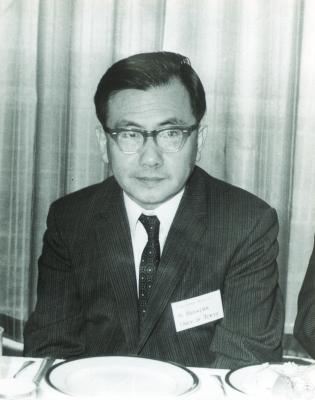
\includegraphics[height=4.8cm]{../assets/Kunihiko_Kodaira.png}
\column{.59\textwidth}
\begin{itemize}
\setlength{\itemsep}{7pt}
\item Born in Tokyo in 1915. In 1949 he moved to the Institute for Advanced Study in Princeton.
\item \textbf{Fields Medal, 1954} (Amsterdam): the first Japanese medallist. Hermann Weyl presented the medal.
\item With Donald Spencer he developed the deformation theory of complex manifolds.
\item Wolf Prize, 1984/85.
\end{itemize}
\par\medskip
His idea: an \textbf{analytic} condition (curvature)
produces an \textbf{algebraic} object (polynomial equations).
\end{columns}
\src{Photo: Konrad Jacobs / MFO, Tokyo 1969, CC BY-SA 2.0 DE. Sources: IAS scholar profile; Encyclopaedia Britannica and MacTutor, ``Kunihiko Kodaira''.}
\end{frame}

\begin{frame}{Where this sits in history}
\begin{center}
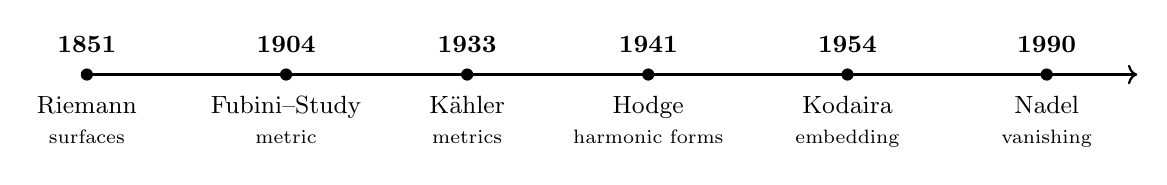
\begin{tikzpicture}[x=1.15cm]
\draw[thick,->] (0,0)--(11.6,0);
\foreach \x/\y/\t/\s in {
 0/1851/Riemann/surfaces,
 2.2/1904/Fubini--Study/metric,
 4.2/1933/Kähler/metrics,
 6.2/1941/Hodge/harmonic forms,
 8.4/1954/Kodaira/embedding,
 10.6/1990/Nadel/vanishing}
{\fill (\x,0) circle (2.2pt);
 \node[above] at (\x,.15) {\small\textbf{\y}};
 \node[below,align=center] at (\x,-.15) {\small \t\\[-1pt]\scriptsize\s};}
\end{tikzpicture}
\end{center}
\par\bigskip
Riemann used analysis to prove that compact Riemann surfaces are algebraic curves.
Kodaira did the same in every dimension.
\end{frame}

\begin{frame}{An embedding needs values and derivatives}
\label{fr:an-embedding-needs-values-10}
\[
\begin{array}{r@{\;}c@{\;}c@{\;}l}
\Phi_{L^N}\colon & X & \longrightarrow & \Pj\bigl(H^0(X,L^N)^*\bigr)\\
& x & \longmapsto & [s_0(x):\cdots:s_M(x)]
\end{array}
\qquad s_0,\ldots,s_M \text{ a basis of } H^0(X,L^N).
\]
\begin{center}
\renewcommand{\arraystretch}{1.4}
\begin{tabular}{ll}
\(\Phi_{L^N}\) is & Language of sections\\
\hline
Defined everywhere & \textbf{Base-point free}: no common zero\\
Injective & \textbf{Separates points}: distinct projective images\\
An immersion & \textbf{Separates tangent directions}
\end{tabular}
\end{center}
\textbf{Separates points:} for every \(x\ne y\), some global section \(s\) satisfies \(s(x)=0\) and \(s(y)\ne0\).
\end{frame}

\begin{frame}{Vanishing lifts prescribed data}
Put \(A=L^N\). For an ideal sheaf \(I\),
\[
0\longrightarrow A\otimes I\longrightarrow A
\longrightarrow A\otimes(\cO_X/I)\longrightarrow0.
\]
The long exact sequence contains
\[
H^0(X,A)\xrightarrow{\ \mathrm{ev}\ } H^0(X,A\otimes\cO_X/I)
\longrightarrow H^1(X,A\otimes I).
\]
\[
\boxed{H^1(X,A\otimes I)=0
\quad\Longrightarrow\quad\mathrm{ev}\text{ is surjective}.}
\]
\begin{center}
\renewcommand{\arraystretch}{1.5}
\begin{tabular}{lll}
Ideal & \(\mathrm{ev}(s)\) & If \(\mathrm{ev}\) is surjective, some section \(s\) has\\
\hline
\(I=\mathfrak m_x\) & \(s(x)\in A|_x\) & \(s(x)\ne0\): \(x\) is not a base point\\
\(I=\mathfrak m_x\cap\mathfrak m_y\) & \(\bigl(s(x),s(y)\bigr)\in A|_x\oplus A|_y\) & \(s(x)=0,\ s(y)\ne0\): \(s\) separates \(x\) and \(y\)
\end{tabular}
\end{center}
\end{frame}

\begin{frame}{The task is a vanishing theorem}
\label{fr:the-task-is-a-12}
We want, for one sufficiently large \(N\),
\(H^1(X,L^N\otimes I)=0\) for three ideals:
\begin{center}
\renewcommand{\arraystretch}{1.6}
\begin{tabular}{lll}
\(I=\mathfrak m_x\) & gives & base-point freeness\\
\(I=\mathfrak m_x\cap\mathfrak m_y\) & gives & point separation\\
\(I=\mathfrak m_x^2\) & gives & tangent separation
\end{tabular}
\end{center}
Kodaira vanishing handles a positive bundle with a canonical twist.
We need a theorem that also allows these ideals.
\end{frame}

\begin{frame}{Kodaira vanishing (1953)}
Let \(X\) be a compact complex manifold, and \(B\) a line bundle with a smooth metric of \textbf{positive} curvature, \(i\Theta_B>0\).
\[
\boxed{H^q(X,K_X\otimes B)=0\qquad(q>0).}
\]
\par\medskip
For us: \(B=L^N\otimes K_X^{-1}\) is positive for \(N\gg0\), so \(H^q(X,L^N)=0\).
But there is no ideal \(I\) yet.
\src{Kodaira, Proc.\ Nat.\ Acad.\ Sci.\ 39 (1953), 1268--1273.}
\end{frame}

\begin{frame}{Hodge theory with values in \(B\)}
\label{fr:hodge-theory-with-values-14}
\textbf{From now on, every form has values in \(B\).}
Split the Chern connection of \((B,h)\) by type: \(\nabla=\partial+\db\). So \(\partial\) and \(\db\) act on \(B\)-valued forms; in a holomorphic frame \(e\),
\(\db(\alpha\otimes e)=(\db\alpha)\otimes e\), with the usual \(\db\) on the right.
\par\medskip
For the smooth proof, \textbf{choose \(\omega=i\Theta_B\)}: it is closed and positive, hence Kähler.
With \(h\) on \(B\), it gives a hermitian product
\((\alpha,\beta)=\int_X\langle\alpha,\beta\rangle\,dV\).
The operators \(\partial^*\) and \(\db^*\) are the formal adjoints:
\[
(\partial\alpha,\beta)=(\alpha,\partial^*\beta),
\qquad
(\db\alpha,\beta)=(\alpha,\db^*\beta).
\]
The Laplacian of \(\db\) is \(\Delta_{\db}=\db\,\db^*+\db^*\db\). Every Dolbeault class has exactly one harmonic representative:
\[
\boxed{H^q(X,\Omega^p_X\otimes B)\ \cong\ \ker\Delta_{\db}.}
\]
For \(p=n\): each class in \(H^q(X,K_X\otimes B)\) is represented by one \(u\) with \(\Delta_{\db}u=0\).
\src{M.~Verbitsky, \emph{Hodge theory}, lecture 16 (2025), slide 4. Huybrechts, \emph{Complex Geometry}, Section 4.1.}
\end{frame}

\begin{frame}{The Bochner--Kodaira--Nakano identity}
\label{fr:the-bochner-kodaira-nakano-15}
There is a second Laplacian, built from \(\partial\):
\[
\Delta_{\partial}=\partial\partial^*+\partial^*\partial .
\]
\textbf{Theorem (Nakano identities).} Let \(\Lambda\) be the adjoint of \(\omega\wedge\), where \(\omega\) is the Kähler form fixed on slide~\hyperlink{fr:hodge-theory-with-values-14}{\pageref{fr:hodge-theory-with-values-14}}. Then
\[
[\Lambda,\db]=-i\,\partial^*,
\qquad
[\Lambda,\partial]=i\,\db^*.
\]
Consequently, with \(\Theta_B\) the curvature of the Chern connection,
\[
\boxed{\Delta_{\db}=\Delta_{\partial}+[\,i\Theta_B\wedge,\Lambda\,].}
\]
\par\medskip
Unlike the scalar case, the two Laplacians differ by a curvature term.
\src{Huybrechts, \emph{Complex Geometry}, Lemma 5.2.3.}
\end{frame}

\begin{frame}{Proof of the Bochner--Kodaira--Nakano identity}
Solve the Nakano identities for the adjoints, with ordinary commutators \([S,T]=ST-TS\):
\[
\db^*=-i\,[\Lambda,\partial],\qquad \partial^*=i\,[\Lambda,\db].
\]
Substitute into \(\Delta_{\db}=\db\,\db^*+\db^*\db\) and \(\Delta_{\partial}=\partial\partial^*+\partial^*\partial\), and expand:
\[
\begin{aligned}
\Delta_{\db}-\Delta_{\partial}
&=-i\bigl(\db\,[\Lambda,\partial]+[\Lambda,\partial]\,\db+\partial[\Lambda,\db]+[\Lambda,\db]\,\partial\bigr)\\
&=-i\bigl(\Lambda\partial\db+\Lambda\db\partial-\db\partial\Lambda-\partial\db\Lambda\bigr)
\;=\;i\,[\,\partial\db+\db\partial,\Lambda\,].
\end{aligned}
\]
The terms \(\db\Lambda\partial\) and \(\partial\Lambda\db\) cancelled.
\par\medskip
Since \(\db^2=0\) (holomorphic) and \(\partial^2=0\) (curvature of type \((1,1)\)),
\[
\partial\db+\db\partial=(\partial+\db)^2=\nabla^2=\Theta_B\wedge,
\qquad\text{hence}\qquad
\boxed{\Delta_{\db}=\Delta_{\partial}+[\,i\Theta_B\wedge,\Lambda\,].}
\]
\end{frame}

\begin{frame}{Proof of Kodaira vanishing}
\label{fr:kv-proof}
Let \(u\) be the harmonic \(B\)-valued \((n,q)\)-form representing a class in \(H^q(X,K_X\otimes B)\).
\par
\textbf{1. Harmonic:} \(\Delta_{\db}u=0\), so \(\int_X\langle\Delta_{\db}u,u\rangle\,dV=0\).
\par
\textbf{2. Bochner--Kodaira--Nakano} (slide~\hyperlink{fr:the-bochner-kodaira-nakano-15}{\pageref{fr:the-bochner-kodaira-nakano-15}}), paired with \(u\) and integrated:
\[
0=\int_X\langle\Delta_{\db}u,u\rangle\,dV
=\int_X\langle\Delta_{\partial}u,u\rangle\,dV
+\int_X\big\langle[\,i\Theta_B\wedge,\Lambda\,]u,u\big\rangle\,dV .
\]
\textbf{3. The first term} (\hyperlink{fr:first-term}{next slide}) is
\(\ \int_X\bigl(|\partial u|^2+|\partial^*u|^2\bigr)\,dV\ \ge0 .\)
\par
\textbf{4. The curvature term.} Our choice \(\omega=i\Theta_B\) makes \(i\Theta_B\wedge\) the Lefschetz operator \(L=\omega\wedge\). On forms of total degree \(k\), \([L,\Lambda]=(k-n)\,\mathrm{id}\). Here \(k=n+q\), so \([\,i\Theta_B\wedge,\Lambda\,]u=q\,u\):
\[
0=\underbrace{\int_X\bigl(|\partial u|^2+|\partial^*u|^2\bigr)\,dV}_{\ge0}
+\;q\int_X|u|^2\,dV .
\]
\textbf{5. Conclusion.} For \(q>0\), this forces \(\int_X|u|^2\,dV=0\), so \(u=0\).
\end{frame}

\begin{frame}{Proof of Kodaira vanishing: why the first term is \(\ge0\)}
\label{fr:first-term}
The first term on the \hyperlink{fr:kv-proof}{previous slide} is \(\displaystyle\int_X\langle\Delta_{\partial}u,u\rangle\,dV=(\Delta_{\partial}u,u)\), in the product of slide~\hyperlink{fr:hodge-theory-with-values-14}{\pageref{fr:hodge-theory-with-values-14}}.
\par\medskip
\textbf{1. Split.} Since \(\Delta_{\partial}=\partial\partial^*+\partial^*\partial\),
\[
(\Delta_{\partial}u,u)=(\partial\partial^*u,u)+(\partial^*\partial u,u).
\]
\textbf{2. Move one operator across.} The rule is \((\partial\alpha,\beta)=(\alpha,\partial^*\beta)\).
\[
(\partial\,\partial^*u,\;u)=(\partial^*u,\;\partial^*u),
\qquad
(\partial^*\,\partial u,\;u)=(\partial u,\;\partial u).
\]
\textbf{3. A form paired with itself is its squared length.}
\[
(\partial^*u,\partial^*u)=\int_X|\partial^*u|^2\,dV,
\qquad
(\partial u,\partial u)=\int_X|\partial u|^2\,dV.
\]
Both integrands are \(\ge0\) at every point, so
\(\displaystyle\int_X\langle\Delta_{\partial}u,u\rangle\,dV=\int_X\bigl(|\partial u|^2+|\partial^*u|^2\bigr)\,dV\ \ge\ 0.\)
\end{frame}

\begin{frame}{What we just proved: Kodaira vanishing}
\label{fr:what-we-just-proved-29}
Let \(X\) be a compact complex manifold, and \(B\) a line bundle with a smooth metric of \textbf{positive} curvature, \(i\Theta_B>0\).
\[
\boxed{H^q(X,K_X\otimes B)=0\qquad(q>0).}
\]
\textbf{The proof in three lines.}
\begin{enumerate}
\item Hodge theory: every class has one harmonic representative \(u\), with \(\Delta_{\db}u=0\).
\item Bochner--Kodaira--Nakano: \(\Delta_{\db}=\Delta_{\partial}+[\,i\Theta_B\wedge,\Lambda\,]\).
\item With \(\omega=i\Theta_B\), the commutator is \(q\,\mathrm{id}\) on \((n,q)\)-forms. Thus \(0\ge q\norm{u}^2\) and \(u=0\).
\end{enumerate}
\par\medskip
For us: \(B=L^N\otimes K_X^{-1}\) is positive for \(N\gg0\), so \(H^q(X,L^N)=0\).
\par\medskip
\textbf{But there is no ideal \(I\) yet.} For the embedding we need vanishing with an ideal sheaf. That is Nadel's theorem.
\end{frame}

\begin{frame}{The solution: Nadel vanishing (1990)}
Let \(X\) be compact Kähler, and \(B\) a line bundle with a \textbf{singular} metric \(h\), \(i\Theta_h\ge\varepsilon\omega\).
The \textbf{multiplier ideal} keeps the germs that stay square-integrable:
\[
\cI(h)_x=\bigl\{f:\ |f|_h^2\ \text{is integrable near}\ x\bigr\}.
\]
\[
\boxed{H^q\bigl(X,K_X\otimes B\otimes\cI(h)\bigr)=0\qquad(q>0).}
\]
Take \(B=L^N\otimes K_X^{-1}\), so \(K_X\otimes B=L^N\).
Different choices of singular metric, which we construct in the proof, make the multiplier ideal
\(\mathfrak m_x\), \(\mathfrak m_x\cap\mathfrak m_y\) or \(\mathfrak m_x^2\).
\src{Nadel, Ann.\ of Math.\ 132 (1990).}
\end{frame}

\begin{frame}{Alan Michael Nadel}
\begin{columns}[c]
\column{.44\textwidth}
\centering

\begin{tikzpicture}
\fill[black!12] (.12,-.12) rectangle (4.32,5.08);
\filldraw[fill=blue!4,draw=blue!50!black] (0,0) rectangle (4.2,5.2);
\draw[blue!50!black,line width=2pt] (.2,0)--(.2,5.2);
\node[align=center,text width=3.6cm] at (2.2,4.65) {\small\textsc{Annals of Mathematics}};
\draw[blue!40] (.6,4.15)--(3.8,4.15);
\node[align=center,text width=3.3cm] at (2.2,3.0) {\small\emph{Multiplier ideal sheaves and Kähler--Einstein metrics of positive scalar curvature}};
\node[align=center] at (2.2,1.5) {\small Alan Michael Nadel};
\node at (2.2,.6) {\Large\textbf{1990}};
\end{tikzpicture}
\column{.52\textwidth}
\begin{itemize}
\setlength{\itemsep}{16pt}
\item His 1990 paper introduced multiplier ideal sheaves while studying \textbf{Kähler--Einstein metrics}.
\item He was a student of \textbf{Yum-Tong Siu} at Harvard: PhD in 1988, with the thesis \emph{Hyperbolic Surfaces}.
\item After the early 1990s the public record stops: we found no later position, no photograph, and no students.
\end{itemize}
\end{columns}
\src{Nadel, Ann. of Math. 132 (1990), 549--596, abstract. Mathematics Genealogy Project, id 175682. Searches of 13 Nov 2026: Oberwolfach Photo Collection, Wikimedia Commons, Wikipedia. Illustration based on the bibliographic record.}
\end{frame}

\begin{frame}{Plan for the rest of today}
\textbf{Goal:} prove Nadel's theorem,
\(\ H^q\bigl(X,K_X\otimes B\otimes\cI(h)\bigr)=0\) for \(q>0\).
\par\medskip
\begin{enumerate}
\setlength{\itemsep}{9pt}
\item \textbf{Singular metrics:} what \(h\) is, and what \(i\Theta_h\ge\varepsilon\omega\) means for it.
\item \textbf{The multiplier ideal \(\cI(h)\):} the definition, and one computation with a logarithmic pole, which produces the ideals \(\mathfrak m_x\) and \(\mathfrak m_x^2\).
\item \textbf{The proof:} keep a fixed smooth Kähler form and derive the lower bound needed to solve the weighted equation.
\end{enumerate}
\par\medskip
\textbf{Next session:} construct singular metrics with prescribed ideals on \(B=L^N\otimes K_X^{-1}\), and deduce the Kodaira embedding theorem.
\src{Following M.~Verbitsky, \emph{Hodge theory}, lecture 23 (2025).}
\end{frame}

\begin{frame}{Reminder: averages over circles}
Let \(f\) be a real function near \(p\in\C\). Its \textbf{average} over the circle of radius \(r\) around \(p\) is
\[
A(r)=\frac{1}{2\pi}\int_0^{2\pi}f(p+re^{i\theta})\,d\theta .
\]
\textbf{Question.} How does the value \(f(p)\) at the centre compare with the averages \(A(r)\)?
\par\medskip
\textbf{Answer,} for smooth \(f\), proved on the \hyperlink{fr:laplacian-appears}{next two slides}:
\begin{itemize}
\setlength{\itemsep}{6pt}
\item if \(\Delta f=0\) (harmonic), then \(f(p)=A(r)\): the value \emph{is} the average;
\item if \(\Delta f\ge0\), then \(f(p)\le A(r)\): the value is \emph{below} the average.
\end{itemize}
\par\medskip
\textbf{Example.} \(f=|z|^2=x^2+y^2\) has \(\Delta f=f_{xx}+f_{yy}=2+2=4\ge0\). Take \(p=0\). On the circle of radius \(r\), \(f\) is constantly \(r^2\), so its average is \(A(r)=r^2\). And \(f(0)=0\). Indeed \(0\le r^2\).
\par\medskip
\textbf{The plan.} First compute \(A'(r)\); the Laplacian appears. Then compare \(A(r)\) with its limit as \(r\to0\).
\end{frame}

\begin{frame}{Why the Laplacian appears in \(A'(r)\)}
\label{fr:laplacian-appears}
\textbf{1. Differentiate under the integral.}
\(\displaystyle A'(r)=\frac{1}{2\pi}\int_0^{2\pi}\frac{\partial}{\partial r}f(p+re^{i\theta})\,d\theta .\)
\par
Moving outward along the ray at angle \(\theta\) is moving along the outward unit normal \(n\) of the circle. So the integrand is the normal derivative \(\nabla f\cdot n\).
\par\medskip
\textbf{2. Write it as an integral over the circle.} The arc length is \(ds=r\,d\theta\), so
\[
A'(r)=\frac{1}{2\pi r}\oint_{|z-p|=r}\nabla f\cdot n\,ds .
\]
This is the \textbf{flux} of the vector field \(\nabla f\) out of the disc, divided by \(2\pi r\).
\par\medskip
\textbf{3. Divergence theorem.} The flux out of a region is the integral of the divergence inside, and \(\operatorname{div}(\nabla f)=f_{xx}+f_{yy}=\Delta f\):
\[
\boxed{A'(r)=\frac{1}{2\pi r}\int_{|z-p|\le r}\Delta f\,dx\,dy .}
\]
\end{frame}

\begin{frame}{From \(A'(r)\) to \(f(p)\le A(r)\)}
\textbf{1. The averages start at \(f(p)\).} Since \(f\) is continuous, \(f(p+se^{i\theta})\to f(p)\) as \(s\to0\), for all \(\theta\) at once. So
\[
A(s)\to f(p)\qquad\text{as } s\to0 .
\]
\textbf{2. If \(\Delta f\ge0\), the averages grow.} By the boxed formula, \(A'(r)\ge0\). So \(A\) is non-decreasing:
\[
A(s)\le A(r)\qquad\text{for } 0<s<r .
\]
\textbf{3. Let \(s\to0\)} in this inequality. The left side tends to \(f(p)\) by step 1:
\[
\boxed{f(p)\le A(r).}
\]
\textbf{4. If \(\Delta f=0\),} then \(A'(r)=0\), so \(A\) is constant, equal to its limit: \(f(p)=A(r)\).
\par\medskip
\textbf{Definition.} An upper semicontinuous \(f:U\to[-\infty,\infty)\) is \textbf{subharmonic} if
\(f(p)\le A(r)\) for every \(p\) and every small circle around \(p\).
For smooth \(f\) this is \(\Delta f\ge0\). The definition needs no derivatives, and it allows the value \(-\infty\): the inequality \(-\infty\le A(r)\) is always true.
\end{frame}

\begin{frame}{The basic example: \(\log|z|\)}
\label{fr:the-basic-example-z-36}
\textbf{1. Away from \(0\) it is harmonic.} Near any \(p\ne0\), \(\log|z|=\operatorname{Re}F\) with \(F=\log z\) holomorphic. Cauchy's formula on the circle around \(p\) says
\[
F(p)=\frac{1}{2\pi}\int_0^{2\pi}F(p+re^{i\theta})\,d\theta .
\]
Take real parts: \(\log|p|\) equals the average \(A(r)\) of \(\log|z|\) over the circle of radius \(r\) around \(p\).
\par\medskip
\textbf{2. At \(0\) it is \(-\infty\).} The average over the circle of radius \(r\) around \(0\) is \(\log r\), and \(-\infty\le\log r\).
\par\medskip
\textbf{3. So \(\log|z|\) is subharmonic on all of \(\C\)}, with one singular point, the pole at \(0\).
\par
\textbf{4. The same argument} works for \(\log|f|\), with \(f\) holomorphic: it is \(\operatorname{Re}\log f\) away from the zeros of \(f\), and \(-\infty\) at the zeros.
\end{frame}

\begin{frame}{Reminder: plurisubharmonic functions}
\textbf{Definition.} A function \(\psi:U\to[-\infty,\infty)\) on an open set \(U\subset\C^n\) is \textbf{plurisubharmonic} (psh) if it is upper semicontinuous and its restriction to every complex line is subharmonic.
\par\medskip
\textbf{1. Smooth case.} A smooth \(\psi\) is psh exactly when \(i\partial\db\psi\ge0\). On a complex line, \(i\partial\db\) is the Laplacian up to a positive factor (slide~\hyperlink{fr:ddbar-laplacian}{\pageref{fr:ddbar-laplacian}}).
\par\medskip
\textbf{2. The basic singular examples.} \(\log|f|\) is psh for \(f\) holomorphic on \(U\). Indeed, restricted to a complex line, \(f\) becomes a holomorphic function \(g\) of one variable, and \(\log|g|\) is subharmonic by item 4 of slide~\hyperlink{fr:the-basic-example-z-36}{\pageref{fr:the-basic-example-z-36}}. Also \(\log|z|\) is psh on \(\C^n\), with value \(-\infty\) at \(0\).
\par\medskip
\textbf{3. Stability.} If \(\psi\) is psh and \(a\ge0\), then \(a\psi\) is psh. A sum of psh functions is psh.
\par\medskip
\textbf{4. Integrability.} On a connected \(U\), a psh function that is not identically \(-\infty\) is locally integrable (slides \hyperlink{fr:log-pole}{\pageref{fr:log-pole}}, \hyperlink{fr:psh-integrable}{\pageref{fr:psh-integrable}}). So \(i\partial\db\psi\) makes sense as a distribution, and it is \(\ge0\).
\src{M.~Verbitsky, \emph{Hodge theory}, lecture 22 (2025); lecture 23, slide 3.}
\end{frame}

\begin{frame}{Why \(i\partial\db\) is the Laplacian on a complex line}
\label{fr:ddbar-laplacian}
\textbf{1. One variable.} Let \(z=x+iy\). Then
\[
\frac{\partial}{\partial z}=\frac12\left(\frac{\partial}{\partial x}-i\frac{\partial}{\partial y}\right),\qquad
\frac{\partial}{\partial\bar z}=\frac12\left(\frac{\partial}{\partial x}+i\frac{\partial}{\partial y}\right),\qquad
\frac{\partial^2f}{\partial z\,\partial\bar z}=\frac14\left(f_{xx}+f_{yy}\right)=\frac14\,\Delta f.
\]
Since \(i\,dz\wedge d\bar z=2\,dx\wedge dy\),
\[
\boxed{i\partial\db f=\frac{\partial^2f}{\partial z\,\partial\bar z}\;i\,dz\wedge d\bar z=\frac12\,\Delta f\;dx\wedge dy.}
\]
So on \(\C\): \(i\partial\db f\ge0\) exactly when \(\Delta f\ge0\).
\par\medskip
\textbf{2. Restrict to a line.} Let \(\psi\) be smooth on \(U\subset\C^n\). On the line \(t\mapsto p+tv\), with \(t\in\C\),
\[
\frac{\partial^2}{\partial t\,\partial\bar t}\,\psi(p+tv)
=\sum_{j,k}\frac{\partial^2\psi}{\partial z_j\,\partial\bar z_k}\,v_j\bar v_k
=\frac14\,\Delta_t\,\psi(p+tv).
\]
\textbf{3. Conclusion.} \(\psi\) is subharmonic on every line exactly when the Hermitian matrix \(\bigl(\partial^2\psi/\partial z_j\partial\bar z_k\bigr)\) is positive semidefinite, that is, when \(i\partial\db\psi\ge0\).
\end{frame}

\begin{frame}{Integrability, an example: polar coordinates \(dx\,dy=t\,dt\,d\theta\)}
\label{fr:polar-coordinates-dx-dy-38}
\begin{columns}[T]
\column{.60\textwidth}
\textbf{1. The coordinates.} Every \(z=x+iy\ne0\) is
\(x=t\cos\theta\), \(y=t\sin\theta\),
with \(t=|z|>0\) the distance to \(0\) and \(\theta\) the angle.
\par
\textbf{2. Change of variables.} An integral in \(x,y\) becomes an integral in \(t,\theta\), multiplied by the determinant of the matrix of partial derivatives:
\[
\det\begin{pmatrix}
\partial x/\partial t&\partial x/\partial\theta\\
\partial y/\partial t&\partial y/\partial\theta
\end{pmatrix}
=\det\begin{pmatrix}
\cos\theta&-t\sin\theta\\
\sin\theta&t\cos\theta
\end{pmatrix}.
\]
\textbf{3. Compute it.}
\(\ t\cos^2\theta+t\sin^2\theta=t\), so \(\ \boxed{dx\,dy=t\,dt\,d\theta}\)
\column{.38\textwidth}
\centering
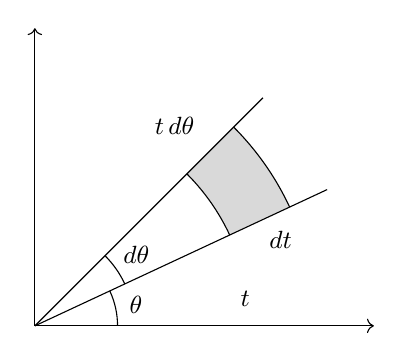
\begin{tikzpicture}[scale=1.05]
\draw[->] (0,0)--(4.1,0);
\draw[->] (0,0)--(0,3.6);
\fill[black!15] (25:2.6)--(25:3.4) arc (25:45:3.4)--(45:2.6) arc (45:25:2.6);
\draw (0,0)--(25:3.9);
\draw (0,0)--(45:3.9);
\draw (25:2.6) arc (25:45:2.6);
\draw (25:3.4) arc (25:45:3.4);
\draw (0:1) arc (0:25:1);
\node at (12:1.25) {\small\(\theta\)};
\node at (35:1.5) {\small\(d\theta\)};
\draw (25:1.2) arc (25:45:1.2);
\node[below right] at (25:3.0) {\small\(dt\)};
\node[above left] at (47:3.0) {\small\(t\,d\theta\)};
\node[below] at (12:2.6) {\small\(t\)};
\end{tikzpicture}
\par\smallskip
{\small The grey region has sides \(dt\) (along the ray) and \(t\,d\theta\) (an arc of the circle of radius \(t\)).}
\end{columns}
\par\smallskip
\textbf{4. Check.} The area of the unit disc:
\(\ \int_0^{2\pi}\!\int_0^1t\,dt\,d\theta=2\pi\cdot\tfrac12=\pi\). Without the factor \(t\) we would get \(2\pi\).
\end{frame}

\begin{frame}{Integrability, an example: the pole of \(\log|z|\)}
\label{fr:log-pole}
\textbf{Claim.} \(\int_{|z|\le1}\log|z|\,dx\,dy\) is finite, although \(\log|z|=-\infty\) at \(0\).
\par
\textbf{1. Polar coordinates} (\hyperlink{fr:polar-coordinates-dx-dy-38}{previous slide}). Here \(\log|z|=\log t\) does not depend on \(\theta\), so
\[
\int_{|z|\le1}\log|z|\,dx\,dy=\int_0^{2\pi}\!\!\int_0^1\log t\cdot t\,dt\,d\theta=2\pi\int_0^1t\log t\,dt .
\]
\textbf{2. The only problem is at \(t=0\),} where \(t\to0\) and \(\log t\to-\infty\). Write the product as a quotient of two functions that blow up:
\(\ t\log t=\dfrac{\log t}{1/t}\).
\par
\textbf{3. L'Hôpital.} Differentiate numerator and denominator:
\[
\frac{(\log t)'}{(1/t)'}=\frac{1/t}{-1/t^2}=-t\ \longrightarrow\ 0
\qquad\text{so}\qquad
t\log t\ \longrightarrow\ 0\quad\text{as } t\to0 .
\]
\textbf{4. Conclusion.} The function \(t\log t\) extends continuously to \([0,1]\), with value \(0\) at \(t=0\). A continuous function on a closed bounded interval has a finite integral.
\end{frame}

\begin{frame}{Integrability in general: psh functions are locally integrable}
\label{fr:psh-integrable}
Let \(U\subset\C^n\) be connected and \(\psi\) psh on \(U\), not identically \(-\infty\). The example \(\log|z|\) of slide~\hyperlink{fr:log-pole}{\pageref{fr:log-pole}} is a special case.
\begin{enumerate}
\item \textbf{Bounded above.} \(\psi\) is upper semicontinuous, so it is bounded above on compact sets. Integrability can only fail if the integral is \(-\infty\).
\item \textbf{Mean value over balls.} For every ball \(B(p,r)\) with closure in \(U\) (proved on slide~\hyperlink{fr:psh-ball-mean}{\pageref{fr:psh-ball-mean}}),
\[
\psi(p)\le\frac{1}{\operatorname{vol}B(p,r)}\int_{B(p,r)}\psi\,dV.
\]
\item \textbf{Finite at \(p\) gives integrable near \(p\).} Let \(B=B(p,r)\) and \(\psi\le M\) on \(B\) (step 1). Then \(M-\psi\ge0\) on \(B\), and by step 2
\[
\int_B(M-\psi)\,dV=M\operatorname{vol}B-\int_B\psi\,dV\le\bigl(M-\psi(p)\bigr)\operatorname{vol}B .
\]
If \(\psi(p)>-\infty\), the right side is finite. So \(M-\psi\) is a non-negative function with finite integral: it is integrable on \(B\), and so is \(\psi=M-(M-\psi)\).
\end{enumerate}
\end{frame}

\begin{frame}{Integrability in general: from one point to all of \(U\)}
\textbf{So far:} if \(\psi(p)>-\infty\), then \(\psi\) is integrable on every ball around \(p\) with closure in \(U\).
\par\smallskip
\textbf{In words:} \(\psi\) cannot be very positive (bounded above), and it cannot be very negative on average (the average is at least \(\psi(p)\)).
\par\medskip
\begin{enumerate}
\setcounter{enumi}{3}
\item \textbf{Spread to all of \(U\).} Let \(W\) be the set of points with a neighbourhood on which \(\psi\) is integrable. \begin{itemize}
\item \(W\) is open, by its definition.
\item \(W\) is nonempty: \(\psi\) is finite at some point, and \hyperlink{fr:psh-integrable}{step 3} applies there.
\item The complement of \(W\) is open. Indeed, if \(q\notin W\), then \(\psi=-\infty\) on a neighbourhood of \(q\): otherwise some \(p'\) near \(q\) has \(\psi(p')>-\infty\), and a ball around \(p'\) contains \(q\). 
\end{itemize}
Since \(U\) is connected, \(W=U\): \(\psi\) is locally integrable on \(U\).
\end{enumerate}
\end{frame}

\begin{frame}{Integrability in general: polar coordinates in \(\C^n\)}
\label{fr:polar-cn}
The next slide integrates over a ball in \(\C^n=\mathbb R^{2n}\), with \(dV\) the usual volume. We need polar coordinates there. We write them around \(0\); around another centre \(p\), replace \(z\) by \(z-p\).
\par\medskip
\textbf{1. The coordinates.} Every \(z\ne0\) is \(z=t\theta\), with \(t=|z|>0\) its distance to \(0\) and \(\theta=z/|z|\) a point of the unit sphere \(S\). The sphere \(S\) has real dimension \(2n-1\).
\par\medskip
\textbf{2. The volume element.} Let \(d\sigma\) be the area measure of \(S\). Then
\[
\boxed{dV=t^{2n-1}\,dt\,d\sigma(\theta).}
\]
Reason: \(t^{2n-1}\) is the Jacobian determinant of the map \((t,\theta)\mapsto t\theta\). Its derivative sends the radial direction \(\partial/\partial t\) to \(\theta\), of length \(1\), and each unit tangent vector \(v\) of \(S\) to \(tv\), of length \(t\). These \(2n\) directions are mutually perpendicular, so the matrix is diagonal with entries \(1,t,\ldots,t\), and its determinant is \(t^{2n-1}\).
\par\medskip
\textbf{3. Check for \(n=1\).} \(S\) is the unit circle, \(d\sigma=d\theta\), the matrix is \(\operatorname{diag}(1,t)\), and we recover \(dx\,dy=t\,dt\,d\theta\) (slide~\hyperlink{fr:polar-coordinates-dx-dy-38}{\pageref{fr:polar-coordinates-dx-dy-38}}).
\end{frame}

\begin{frame}{Integrability in general: the mean value inequality over balls}
\label{fr:psh-ball-mean}
\textbf{Claim.} If \(\psi\) is psh, then \(\psi(p)\operatorname{vol}B(p,r)\le\int_{B(p,r)}\psi\,dV\). Here \(S\), \(d\sigma\) are as on the \hyperlink{fr:polar-cn}{previous slide}.
\begin{enumerate}
\item \textbf{One line.} Each complex line through \(p\) is \(\{p+tv:\ t\in\C\}\) for some \(v\in S\); then \(|t|\) is the distance to \(p\). On this line \(\psi\) is subharmonic in \(t\), so for \(s<r\):
\[
\psi(p)\le\frac{1}{2\pi}\int_0^{2\pi}\psi(p+se^{i\theta}v)\,d\theta .
\]
\item \textbf{All directions.} Integrate over \(v\in S\). For each \(\theta\), the map \(v\mapsto e^{i\theta}v\) is a rotation of \(S\), and \(d\sigma\) is rotation-invariant, so the integral over \(S\) does not depend on \(\theta\):
\[
\psi(p)\,\sigma(S)\le\int_S\psi(p+sv)\,d\sigma(v).
\]
\item \textbf{All radii.} Multiply by \(s^{2n-1}\) and integrate over \(0<s<r\). Since \(dV=s^{2n-1}\,ds\,d\sigma\), the right side becomes \(\int_{B(p,r)}\psi\,dV\), and the left side \(\psi(p)\int_0^r\!\!\int_S s^{2n-1}\,d\sigma\,ds=\psi(p)\operatorname{vol}B(p,r)\).
\end{enumerate}
All integrals are numbers or \(-\infty\), since \(\psi\) is bounded above.
\end{frame}

\begin{frame}{Singular metrics: the definition}
\label{fr:singular-def}
\textbf{Definition 1.} A function \(f:X\to[-\infty,\infty)\) is \textbf{almost plurisubharmonic} if near every point
\(\ f=(\text{a psh function})+(\text{a smooth function}).\)
\par
The two pieces may change from one neighbourhood to another; \(f\) itself is one function on all of \(X\).
\par\medskip
\textbf{Definition 2.} Let \(h_0\) be a smooth hermitian metric on \(B\), and \(f\) an almost psh function. Then
\(\ \boxed{h=h_0\,e^{-2f}}\ \)
is called a \textbf{singular metric} on \(B\).
\par\medskip
\textbf{1. Nothing is glued.} Both \(h_0\) and \(f\) are defined on all of \(X\), and \(h\) is their product.
\par
\textbf{2. Where is it singular?} Where \(f=-\infty\): there \(e^{-2f}=+\infty\), and every nonzero vector of \(B\) has infinite length. Elsewhere \(h\) is an honest metric on the fibres.
\par
\textbf{3. Why ``almost''?} On a compact \(X\), a psh function is constant (not proved here). So we can only ask for psh locally, up to a smooth correction.
\src{M.~Verbitsky, \emph{Hodge theory}, lecture 23 (2025), slide 2.}
\end{frame}

\begin{frame}{Singular metrics: local form, curvature, positivity}
Let \(h=h_0e^{-2f}\) be a singular metric on \(B\) (\hyperlink{fr:singular-def}{Definition 2}): \(h_0\) is a smooth metric on \(B\), and \(f\) is almost psh.
\par\medskip
\textbf{1. Locally, a singular metric is \(e^{-2\varphi}\) with \(\varphi\) almost psh.} Let \(e\) be a holomorphic frame of \(B\). Write \(|e|_{h_0}^2=e^{-2\varphi_0}\), with \(\varphi_0\) smooth. Then
\[
|e|_h^2=e^{-2\varphi_0}\,e^{-2f}=e^{-2\varphi},
\qquad \varphi=\varphi_0+f .
\]
So \(\varphi\) is again (psh) + (smooth), and \(\varphi=-\infty\) exactly where \(f=-\infty\).
\par
\textbf{2. Curvature.} For a smooth metric, \(i\Theta=2i\,\partial\db\varphi\). For a singular metric we \emph{define} the curvature by the same formula,
\(\ i\Theta_h=2i\,\partial\db\varphi\),
with the derivatives taken as distributions. This makes sense because \(\varphi\) is locally integrable.
\par
\textbf{3. Positivity.} Write \(\omega=i\partial\db\rho\) locally, with \(\rho\) smooth. We \emph{define}:
\[
i\Theta_h\ge\varepsilon\omega
\quad\Longleftrightarrow\quad
\varphi-\tfrac{\varepsilon}{2}\rho\ \text{ is plurisubharmonic.}
\]
For smooth \(\varphi\) this is the usual inequality between smooth forms.
\src{M.~Verbitsky, \emph{Hodge theory}, lecture 23 (2025), slide 2.}
\end{frame}

\begin{frame}{The multiplier ideal}
Let \(h\) be a singular metric on \(B\), with \(|e|_h^2=e^{-2\varphi}\) in a holomorphic frame \(e\) near \(x\).
\[
\boxed{\cI(h)_x=\Bigl\{f\in\cO_{X,x}:\ \int_U|f|^2e^{-2\varphi}\,dV<\infty\ \text{for some neighbourhood } U \text{ of } x\Bigr\}.}
\]
\textbf{1. It is an ideal.} If \(f\in\cI(h)_x\) and \(g\) is holomorphic near \(x\), then \(g\) is bounded near \(x\), so \(|gf|^2e^{-2\varphi}\) is still integrable.
\par\medskip
\textbf{2. It does not depend on the frame.} Another frame changes \(\varphi\) by a smooth function, which is bounded near \(x\).
\par\medskip
\textbf{3. Where \(\varphi\) is bounded, nothing happens:} \(\cI(h)_x=\cO_{X,x}\). The ideal only sees the points where \(\varphi=-\infty\).
\par\medskip
\textbf{4. Meaning.} A section \(s=fe\) of \(B\) has \(|s|_h^2=|f|^2e^{-2\varphi}\). So \(B\otimes\cI(h)\) is the sheaf of holomorphic sections of \(B\) that are locally square-integrable for \(h\).
\src{M.~Verbitsky, \emph{Hodge theory}, lecture 23 (2025), slide 2.}
\end{frame}

\begin{frame}{Example: a logarithmic pole}
\label{fr:example-a-logarithmic-pole-43}
\textbf{The bundle.} The trivial line bundle on \(\C^n\). A section is just a function \(u\).
\par\medskip
\textbf{The singular metric.} In \hyperlink{fr:singular-def}{Definition 2}, take \(h_0\) the standard metric: the frame \(1\) has length \(|1|_{h_0}=1\), so every section has \(|u|_{h_0}^2=|u|^2\). Take
\(\ f=\varphi=a\log|z|\), with \(a>0\); it is psh, so in particular almost psh. The singular metric is \(h=h_0e^{-2f}\):
\[
|u|_h^2=|u|_{h_0}^2\,e^{-2f}=|u|^2\,e^{-2\varphi}=\frac{|u|^2}{|z|^{2a}} .
\]
\textbf{Where is it singular?} Only at \(0\), where \(\varphi=-\infty\). Away from \(0\) the multiplier ideal is all of \(\cO\).
\par\medskip
\textbf{The question: what is the multiplier ideal at \(0\)?} By definition, it consists of the holomorphic germs \(u\) at \(0\) with
\(\ \displaystyle\int_{B_1(0)}\frac{|u|^2}{|z|^{2a}}\,dV<\infty\).
The answer depends on \(a\), and on how fast \(u\) vanishes at \(0\).
\src{M.~Verbitsky, \emph{Hodge theory}, lecture 23 (2025), slide 3.}
\end{frame}

\begin{frame}{Step 1: polar coordinates in our integral}
\label{fr:ex-step1-applied}
\textbf{1. Rewrite the integrand} in the polar coordinates \(z=t\theta\) of slide~\hyperlink{fr:polar-cn}{\pageref{fr:polar-cn}}. Since \(|z|=t\),
\[
\frac{|u(z)|^2}{|z|^{2a}}=\frac{|u(t\theta)|^2}{t^{2a}} .
\]
\textbf{2. The unit ball} \(B_1(0)\) is described by \(0<t<1\) and \(\theta\in S\).
\par\medskip
\textbf{3. Use \(dV=t^{2n-1}\,dt\,d\sigma\).}
\[
\int_{B_1(0)}\frac{|u|^2}{|z|^{2a}}\,dV
=\int_0^1\!\!\int_S\frac{|u(t\theta)|^2}{t^{2a}}\;t^{2n-1}\,d\sigma(\theta)\,dt .
\]
\textbf{4. Collect the powers of \(t\).} They do not depend on \(\theta\), so they come out of the inner integral:
\[
\boxed{\int_{B_1(0)}\frac{|u|^2}{|z|^{2a}}\,dV
=\int_0^1t^{\,2n-1-2a}\Bigl(\int_S|u(t\theta)|^2\,d\sigma(\theta)\Bigr)dt .}
\]
\textbf{What is left.} At \(t=0\) the power \(t^{\,2n-1-2a}\) can blow up. The inner integral can cancel this, if it tends to \(0\) fast enough as \(t\to0\).
\end{frame}

\begin{frame}{Step 2: how \(u\) behaves on small spheres}
\label{fr:step-how-u-behaves-46}
We need \(\int_S|u(t\theta)|^2\,d\sigma\) for small \(t\).
\par
\textbf{1. Taylor expansion at \(0\).} Group the terms by degree:
\[
u=P_k+P_{k+1}+P_{k+2}+\cdots,
\]
with \(P_j\) a homogeneous polynomial of degree \(j\), and \(P_k\ne0\) the first one that is not zero. The number \(k\) is the \textbf{order of vanishing} of \(u\) at \(0\).
\par\smallskip
\textbf{2. Examples.} \(u(0)\ne0\): \(k=0\). \(\ u=z_1\): \(k=1\). \(\ u=z_1z_2\) or \(u=z_1^2\): \(k=2\).
\par\smallskip
\textbf{3. Homogeneous means} \(P_j(t\theta)=t^{\,j}P_j(\theta)\). So
\[
u(t\theta)=t^{\,k}P_k(\theta)+t^{\,k+1}P_{k+1}(\theta)+\cdots,
\qquad
|u(t\theta)|^2=t^{\,2k}|P_k(\theta)|^2+O(t^{\,2k+1}).
\]
\textbf{4. Integrate over the sphere.}
\[
\int_S|u(t\theta)|^2\,d\sigma=A\,t^{\,2k}+O(t^{\,2k+1}),
\qquad A=\int_S|P_k|^2\,d\sigma .
\]
The number \(A\) is \(>0\): if \(P_k=0\) on all of \(S\), then \(P_k(t\theta)=t^{\,k}P_k(\theta)=0\) everywhere.
\end{frame}

\begin{frame}{Step 3: put steps 1 and 2 together}
\label{fr:ex-step3}
\textbf{Where we are.} A holomorphic \(u\) is in the multiplier ideal at \(0\) exactly when \(\int_{B_1(0)}\frac{|u|^2}{|z|^{2a}}\,dV\) is finite. We are finding out when that happens.
\par\medskip
\textbf{1. From \hyperlink{fr:ex-step1-applied}{step 1},} with \(I(t)=\int_S|u(t\theta)|^2\,d\sigma\):
\[
\int_{B_1(0)}\frac{|u|^2}{|z|^{2a}}\,dV=\int_0^1t^{\,2n-1-2a}\,I(t)\,dt .
\]
\textbf{2. From \hyperlink{fr:step-how-u-behaves-46}{step 2},} \(\ I(t)=A\,t^{\,2k}+O(t^{\,2k+1})=A\,t^{\,2k}\bigl(1+O(t)\bigr)\), with \(A>0\).
\par\medskip
\textbf{3. Multiply.} Add the exponents \(2n-1-2a\) and \(2k\):
\[
t^{\,2n-1-2a}\,I(t)=A\,t^{\,c}\bigl(1+O(t)\bigr),
\qquad c=2k+2n-1-2a .
\]
\textbf{4. For small \(t\) the factor \(1+O(t)\) is close to \(1\),} say between \(\tfrac12\) and \(2\) for \(0<t<\delta\). So there
\[
\boxed{\tfrac12A\,t^{\,c}\ \le\ t^{\,2n-1-2a}\,I(t)\ \le\ 2A\,t^{\,c}.}
\]
\end{frame}

\begin{frame}{Step 3, continued: only \(t\to0\) matters}
Write \(g(t)=t^{\,2n-1-2a}\,I(t)\ge0\). We want to know whether \(\int_0^1g(t)\,dt\) is finite.
\par
\textbf{1. Cut the interval in two,} at the \(\delta\) of the \hyperlink{fr:ex-step3}{previous slide}:
\[
\int_0^1g(t)\,dt=\int_0^\delta g(t)\,dt+\int_\delta^1g(t)\,dt .
\]
\textbf{2. The piece away from \(0\) is always finite.} On \([\delta,1]\) neither factor of \(g\) blows up:
\begin{itemize}
\item \(t^{\,2n-1-2a}\) can only be infinite at \(t=0\), and here \(t\ge\delta>0\);
\item \(I(t)=\int_S|u(t\theta)|^2\,d\sigma\le\operatorname{Vol}(S)\cdot\max|u|^2\), because \(u\) is continuous on the closed ball.
\end{itemize}
So \(g\le K\) on \([\delta,1]\) for some constant \(K\), and
\(\ \int_\delta^1g(t)\,dt\le K\,(1-\delta)<\infty .\)
\par\medskip
\textbf{3. So everything is decided by the piece near \(0\):}
\[
\int_0^1g(t)\,dt<\infty\quad\Longleftrightarrow\quad\int_0^\delta g(t)\,dt<\infty .
\]
\end{frame}

\begin{frame}{Step 3, conclusion: compare with \(t^{\,c}\)}
\label{fr:step-conclusion-compare-with-49}
\textbf{1. The squeeze.} For every \(t\) in \((0,\delta)\),
\[
\tfrac12A\,t^{\,c}\ \le\ g(t)\ \le\ 2A\,t^{\,c}.
\]
\textbf{2. Integrate it.} A smaller function has a smaller integral, and constants come out:
\[
\tfrac12A\int_0^\delta t^{\,c}\,dt\ \le\ \int_0^\delta g(t)\,dt\ \le\ 2A\int_0^\delta t^{\,c}\,dt .
\]
\textbf{3. Read it.}
\begin{itemize}
\item If \(\int_0^\delta t^{\,c}\,dt\) is finite, the right inequality makes \(\int_0^\delta g\) finite.
\item If \(\int_0^\delta t^{\,c}\,dt\) is infinite, the left inequality makes \(\int_0^\delta g\) infinite.
\end{itemize}
\textbf{4. Conclusion.} The same cut shows that \(\int_0^\delta t^{\,c}\,dt\) and \(\int_0^1t^{\,c}\,dt\) are finite together. So
\[
\boxed{u \text{ is in the multiplier ideal at } 0
\quad\Longleftrightarrow\quad
\int_0^{1}t^{\,c}\,dt<\infty ,\qquad c=2k+2n-1-2a .}
\]
\end{frame}

\begin{frame}{Step 4: when is \(\int_0^1t^{\,c}\,dt\) finite?}
\label{fr:step-when-is-t-50}
\textbf{1. Compute with a cutoff:} integrate from a small \(\eta>0\), not from \(0\), since \(t^{\,c}\) may be infinite at \(0\). The integral from \(0\) is the limit as \(\eta\to0\).
\par
\textbf{2. The case \(c\ne-1\).} An antiderivative of \(t^{\,c}\) is \(\frac{t^{\,c+1}}{c+1}\). Evaluate it at \(1\) and at \(\eta\):
\[
\int_\eta^1t^{\,c}\,dt=\Bigl[\frac{t^{\,c+1}}{c+1}\Bigr]_\eta^1=\frac{1-\eta^{\,c+1}}{c+1}.
\]
Now let \(\eta\to0\):
\begin{itemize}
\item if \(c+1>0\), then \(\eta^{\,c+1}\to0\), and the limit is the finite number \(\frac{1}{c+1}\);
\item if \(c+1<0\), then \(\eta^{\,c+1}\to\infty\), and the integral diverges.
\end{itemize}
\textbf{3. The borderline case \(c=-1\).} Now \(t^{\,c}=\frac1t\), and the power rule fails. The antiderivative is \(\log t\):
\(\ \int_\eta^1\frac{dt}{t}=\log1-\log\eta=-\log\eta\to\infty\) as \(\eta\to0\). It diverges too.
\par
\textbf{4. Conclusion.}\quad
\(\boxed{\int_0^1t^{\,c}\,dt \text{ is finite exactly when } c>-1 .}\)
\end{frame}

\begin{frame}{The answer: \(k>a-n\)}
\textbf{1. What we know.}
\begin{itemize}
\item Slide~\hyperlink{fr:step-conclusion-compare-with-49}{\pageref{fr:step-conclusion-compare-with-49}}: \(u\) is in the multiplier ideal at \(0\) exactly when \(\int_0^1t^{\,c}\,dt\) is finite, where \(c=2k+2n-1-2a\).
\item Slide~\hyperlink{fr:step-when-is-t-50}{\pageref{fr:step-when-is-t-50}}: \(\int_0^1t^{\,c}\,dt\) is finite exactly when \(c>-1\).
\end{itemize}
\textbf{2. Substitute \(c=2k+2n-1-2a\).}
\[
c>-1
\iff 2k+2n-1-2a>-1
\iff 2k+2n-2a>0
\iff k>a-n .
\]
\textbf{3. The answer.}\quad
\(\boxed{u \text{ is in the multiplier ideal at } 0
\quad\Longleftrightarrow\quad k>a-n .}\)
\par\medskip
\textbf{Reminder of the letters.}
\begin{itemize}
\item \(k\) is the order of vanishing of \(u\) at \(0\) (slide~\hyperlink{fr:step-how-u-behaves-46}{\pageref{fr:step-how-u-behaves-46}});
\item \(a\) is the exponent we chose in the metric: \(\varphi=a\log|z|\), so \(|u|_h^2=|u|^2/|z|^{2a}\) (slide~\hyperlink{fr:example-a-logarithmic-pole-43}{\pageref{fr:example-a-logarithmic-pole-43}}). A larger \(a\) is a more singular metric;
\item \(n\) is the complex dimension.
\end{itemize}
\src{M.~Verbitsky, \emph{Hodge theory}, lecture 23 (2025), slides 3 and 4.}
\end{frame}

\begin{frame}{Which germs survive?}
\[
\boxed{u\in\cI(h)_0\quad\Longleftrightarrow\quad u \text{ vanishes at } 0 \text{ to order } k>a-n .}
\]
\begin{center}
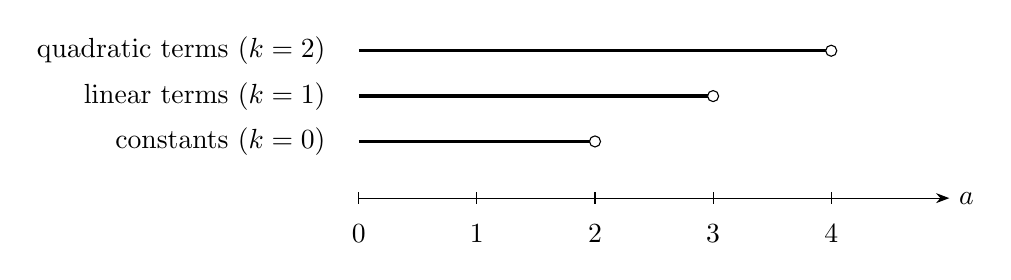
\begin{tikzpicture}[x=1.5cm,y=.72cm]
\draw[-{Stealth}] (1,0)--(6,0) node[right] {\(a\)};
\foreach \x/\lab in {1/0,2/1,3/2,4/3,5/4} {
 \draw (\x,.1)--(\x,-.1) node[below=4pt] {\(\lab\)};}
\node[anchor=east] at (.8,1) {constants (\(k=0\))};
\draw[very thick] (1,1)--(3,1); \draw[fill=white] (3,1) circle (2pt);
\node[anchor=east] at (.8,1.8) {linear terms (\(k=1\))};
\draw[very thick] (1,1.8)--(4,1.8); \draw[fill=white] (4,1.8) circle (2pt);
\node[anchor=east] at (.8,2.6) {quadratic terms (\(k=2\))};
\draw[very thick] (1,2.6)--(5,2.6); \draw[fill=white] (5,2.6) circle (2pt);
\end{tikzpicture}
\end{center}
Picture for \(n=2\): a germ of order \(k\) survives for \(a\) on its bar, \(a<k+2\).
\par\medskip
\textbf{Conclusion.} A more singular metric (larger \(a\)) has a smaller multiplier ideal: as \(a\) grows, first the constants drop out, then the linear terms, then the quadratic ones.
\src{M.~Verbitsky, \emph{Hodge theory}, lecture 23 (2025), slides 3 and 4.}
\end{frame}

\begin{frame}{Which ideals appear?}
\label{fr:which-ideals}
The criterion is \(k>a-n\), and the order of vanishing \(k\) is a whole number. So the condition changes only when \(a-n\) passes a whole number.
\begin{center}
\renewcommand{\arraystretch}{1.4}
\begin{tabular}{llll}
Range of \(a\) & So \(a-n\) is in & \(k>a-n\) means & \(\cI(h)_0\)\\
\hline
\(a<n\) & \((-\infty,0)\) & \(k\ge0\): no condition & \(\cO\)\\
\(n\le a<n+1\) & \([0,1)\) & \(k\ge1\): \(u(0)=0\) & \(\mathfrak m_0\)\\
\(n+1\le a<n+2\) & \([1,2)\) & \(k\ge2\): \(u(0)=0\) and all \(\frac{\partial u}{\partial z_j}(0)=0\) & \(\mathfrak m_0^2\)
\end{tabular}
\end{center}
In general, for \(a\ge n\): \(\ \cI(h)_0=\mathfrak m_0^{\,\lfloor a-n\rfloor+1}\).
\par\medskip
The last column uses: \(k\ge1\) exactly when \(u\in\mathfrak m_0\), and \(k\ge2\) exactly when \(u\in\mathfrak m_0^2\). The next two slides explain these two ideals.
\par\medskip
\textbf{Why we care.} Choosing \(a\) produces exactly the ideals needed for the embedding.
\src{M.~Verbitsky, \emph{Hodge theory}, lecture 23 (2025), slides 3 and 4.}
\end{frame}

\begin{frame}{Some algebra: the ideal \(\mathfrak m_0\)}
\label{fr:ideal-m0}
Let \(\cO\) be the ring of germs of holomorphic functions at \(0\in\C^n\).
\par
\textbf{1. The maximal ideal.} \(\ \mathfrak m_0=\{u\in\cO:\ u(0)=0\}\): the germs with order of vanishing \(k\ge1\).
\par
\textbf{2. One variable.} If \(u(0)=0\), the power series has no constant term:
\[
u=c_1z+c_2z^2+\cdots=z\,(c_1+c_2z+\cdots)=z\,g(z),\qquad g(0)=c_1=u'(0).
\]
\textbf{3. Several variables.} If \(u(0)=0\), every monomial of the power series contains some \(z_i\). Pull out one variable from each monomial and collect:
\[
\boxed{u=z_1g_1+\cdots+z_ng_n,}\qquad g_i \text{ holomorphic}.
\]
\textbf{4. Example,} \(n=2\): \(\ u=z_1+z_1z_2+z_2^2=z_1(1+z_2)+z_2\,(z_2)\). So \(g_1=1+z_2\), \(g_2=z_2\).
\par\vspace{-1pt}
\textbf{5. The value \(g_i(0)\)} is the coefficient of the monomial \(z_i\) in \(u\), that is,
\(\ g_i(0)=\frac{\partial u}{\partial z_i}(0)\).
In the example: \(g_1(0)=1\), \(g_2(0)=0\).
\par
\textbf{6. Meaning.} \(\mathfrak m_0\) is generated by the coordinates \(z_1,\ldots,z_n\).
\end{frame}

\begin{frame}{Some algebra: the ideal \(\mathfrak m_0^2\)}
\textbf{1. Definition.} \(\mathfrak m_0^2\) is the ideal generated by the products \(fg\) with \(f,g\in\mathfrak m_0\). Its elements are finite sums of such products. It is generated by the \(z_iz_j\).
\par\medskip
\textbf{2. Claim.} \(\ \mathfrak m_0^2=\{u:\ u(0)=0 \text{ and all first derivatives of } u \text{ vanish at } 0\}\): the germs with order of vanishing \(k\ge2\).
\par\medskip
\textbf{3. Why ``\(\supset\)''.} Let \(u(0)=0\), with all first derivatives zero at \(0\). By the \hyperlink{fr:ideal-m0}{previous slide},
\[
u=z_1g_1+\cdots+z_ng_n,\qquad g_i(0)=\frac{\partial u}{\partial z_i}(0)=0 .
\]
So each \(g_i\) is in \(\mathfrak m_0\), and \(u\) is a sum of products \(z_i\cdot g_i\) of two elements of \(\mathfrak m_0\).
\par
\textbf{4. Why ``\(\subset\)''.} If \(f(0)=g(0)=0\), then \(fg\) vanishes at \(0\), and by the product rule
\(\ \partial_i(fg)(0)=\partial_if(0)\,g(0)+f(0)\,\partial_ig(0)=0\).
\par\medskip
\textbf{5. In general,} \(\ \boxed{\mathfrak m_0^{\,j}=\{u:\ k\ge j\}}\), where \(k\) is the order of vanishing of \(u\) at \(0\).
\par\medskip
\textbf{6. So the answer \(k>a-n\) is an ideal:} a power of \(\mathfrak m_0\), as on the bar diagram.
\end{frame}

\begin{frame}{Nadel vanishing: the statement again}
Let \((X,\omega)\) be a compact Kähler manifold, and \(B\) a line bundle with a \textbf{singular} metric \(h\) such that \(i\Theta_h\ge\varepsilon\omega\) for some \(\varepsilon>0\).
\[
\boxed{H^q\bigl(X,K_X\otimes B\otimes\cI(h)\bigr)=0\qquad(q>0).}
\]
\textbf{Compare with Kodaira vanishing.}
\begin{itemize}
\setlength{\itemsep}{6pt}
\item If \(h\) is smooth, then \(\cI(h)=\cO_X\), and this is Kodaira vanishing (slide~\hyperlink{fr:what-we-just-proved-29}{\pageref{fr:what-we-just-proved-29}}).
\item Now fix a smooth Kähler form \(\omega\). Since \(h\) is singular, its curvature need not be a smooth form, so we cannot choose it as our Kähler form.
\item The price of the singularities is the ideal \(\cI(h)\): only square-integrable sections are controlled.
\end{itemize}
\src{Nadel, Ann.\ of Math.\ 132 (1990). M.~Verbitsky, \emph{Hodge theory}, lecture 23 (2025), slide 12.}
\end{frame}

\begin{frame}{Proof, step 1: square-integrable forms}
\label{fr:nadel-step1}
From now on, forms are \(B\)-valued \((n,q)\)-forms, and lengths are measured with \(h\) and \(\omega\).
\par\smallskip
\textbf{Definition.} A form \(u\) with measurable coefficients is \textbf{locally \(L^2\)} if, on every open set \(U\) with compact closure,
\[
\int_U|u|_h^2\,dV<\infty
\qquad\text{and}\qquad
\int_U|\db u|_h^2\,dV<\infty ,
\]
where \(\db u\) is computed \textcolor{red}{in the sense of distributions.}\textsuperscript{*}
\par\smallskip
Let \(\mathcal L^{n,q}\) be the sheaf of locally \(L^2\) forms of type \((n,q)\).
\par\medskip
\textbf{In degree \(0\).} A form \(u\in\mathcal L^{n,0}\) with \(\db u=0\) is holomorphic (elliptic regularity), so it is a holomorphic section of \(K_X\otimes B\) that is locally square-integrable for \(h\). That is:
\[
{\color{red}\ker\bigl(\db:\mathcal L^{n,0}\to\mathcal L^{n,1}\bigr)=K_X\otimes B\otimes\cI(h).}
\]
\src{\textsuperscript{*}\,\textcolor{red}{Red} means: I did not verify this.\\
M.~Verbitsky, \emph{Hodge theory}, lecture 23 (2025), slides 9 and 10.}
\end{frame}

\begin{frame}{Proof, step 2: an \(L^2\) Dolbeault resolution}
\label{fr:nadel-step2}
\[
0\longrightarrow K_X\otimes B\otimes\cI(h)
\longrightarrow\mathcal L^{n,0}\xrightarrow{\ \db\ }\mathcal L^{n,1}
\xrightarrow{\ \db\ }\mathcal L^{n,2}\xrightarrow{\ \db\ }\cdots
\]
\textbf{1. It is exact at \(\mathcal L^{n,0}\):} the \hyperlink{fr:nadel-step1}{previous slide}.
\par
\textbf{2. It is exact at \(\mathcal L^{n,q}\), \(q>0\):} this is the \textcolor{red}{\textbf{\(L^2\) Poincaré lemma}}. On a small ball, every locally \(L^2\) form \(\eta\) with \(\db\eta=0\) is \(\eta=\db\alpha\) with \(\alpha\) locally \(L^2\). We take it as an analytic input.
\par
\textbf{3. \textcolor{red}{The sheaves \(\mathcal L^{n,q}\) are fine}:} if \(\chi\) is a smooth cutoff and \(u\) is locally \(L^2\), then so is \(\chi u\), because
\(\ \db(\chi u)=\db\chi\wedge u+\chi\,\db u .\)
\par\medskip
\textbf{4. Conclusion,} exactly as for the usual Dolbeault resolution:
\[
H^q\bigl(X,K_X\otimes B\otimes\cI(h)\bigr)
=\frac{\ker\bigl(\db:\ L^2\text{ forms of type }(n,q)\bigr)}{\operatorname{im}\bigl(\db:\ L^2\text{ forms of type }(n,q-1)\bigr)} .
\]
On the compact \(X\), locally \(L^2\) is the same as \(L^2\).
\src{M.~Verbitsky, \emph{Hodge theory}, lecture 23 (2025), slides 10 and 11.}
\end{frame}

\begin{frame}{Proof, step 3: a lemma about Hilbert spaces}
\label{fr:nadel-step3}
\textcolor{red}{\textbf{Lemma.}} Let \(H_1\xrightarrow{\ T\ }H_2\xrightarrow{\ S\ }H_3\) be closed, densely defined operators between Hilbert spaces, with \(S\circ T=0\). Suppose there is \(C>0\) with
\[
\norm{T^*x}^2+\norm{Sx}^2\ \ge\ C\,\norm{x}^2
\qquad\text{for all } x\in\operatorname{Dom}S\cap\operatorname{Dom}T^* .
\]
Then \(\operatorname{im}T=\ker S\).
\par\medskip
\textbf{Why the estimate helps.} Let \(x\in\ker S\) be orthogonal to \(\operatorname{im}T\).
\begin{enumerate}
\item Orthogonal to \(\operatorname{im}T\) means \((Ty,x)=0\) for all \(y\); that is, \(T^*x=0\).
\item So \(C\norm{x}^2\le\norm{T^*x}^2+\norm{Sx}^2=0\), and \(x=0\).
\item Hence \(\operatorname{im}T\) is dense in \(\ker S\). The estimate also shows that \(\operatorname{im}T\) is closed.
\end{enumerate}
\par\medskip
This is the Hilbert space form of ``a harmonic form must vanish''.
\src{M.~Verbitsky, \emph{Hodge theory}, lecture 23 (2025), slide 5 (Theorem 1); proof in lecture 17.}
\end{frame}

\begin{frame}{Proof, step 4: the estimate for Nadel}
\label{fr:apply-estimate}
\textbf{Bochner--Kodaira--Nakano} (slide~\hyperlink{fr:the-bochner-kodaira-nakano-15}{\pageref{fr:the-bochner-kodaira-nakano-15}}): \(\ \Delta_{\db}=\Delta_{\partial}+[\,i\Theta_h\wedge,\Lambda\,]\).
\par\medskip
Pair with an \((n,q)\)-form \(u\), integrate over \(X\), and integrate by parts:
\[
\begin{aligned}
\norm{\db u}^2+\norm{\db^*u}^2
&=\underbrace{\int_X\bigl(|\partial u|^2+|\partial^*u|^2\bigr)\,dV}_{\ge0}
+\underbrace{\int_X\big\langle[\,i\Theta_h\wedge,\Lambda\,]u,u\big\rangle\,dV}_{\ge q\varepsilon\int_X|u|^2dV}.
\end{aligned}
\]
So \(\ \boxed{\norm{\db^*u}^2+\norm{\db u}^2\ge q\varepsilon\norm{u}^2.}\)
\par\smallskip
As for Kodaira (slide~\hyperlink{fr:kv-proof}{\pageref{fr:kv-proof}}), but for any \(L^2\) form \(u\), and with \(\ge q\varepsilon\) in place of \(=q\).
\par\smallskip
\textcolor{red}{\textbf{Two inputs we do not prove.}}
\begin{enumerate}
\item The identity can be used for \(L^2\) forms and a singular \(h\).
\item The bound \(q\varepsilon\). For smooth \(h\) see \href{https://github.com/danimalabares/tmp/blob/main/kodaira-lectures/archive/curvature-inequality/curvature-inequality.pdf}{\textcolor{blue}{\underline{these slides}}}.
\end{enumerate}
\src{M.~Verbitsky, \emph{Hodge theory}, lecture 23 (2025), slides 11 and 12.}
\end{frame}

\begin{frame}{Nadel vanishing: conclusion}
\begin{enumerate}
\setlength{\itemsep}{8pt}
\item \textbf{Resolution} (\hyperlink{fr:nadel-step2}{step 2}): a class in \(H^q\bigl(X,K_X\otimes B\otimes\cI(h)\bigr)\) is represented by an \(L^2\) form \(f\) of type \((n,q)\) with \(\db f=0\).
\item \textbf{Estimate} (\hyperlink{fr:apply-estimate}{step 4}): \(\norm{\db^*u}^2+\norm{\db u}^2\ge q\varepsilon\norm{u}^2\).
\item \textbf{Lemma} (\hyperlink{fr:nadel-step3}{step 3}), applied to
\[
\underbrace{L^2\ (n,q-1)\text{-forms}}_{H_1}\xrightarrow{\ T=\db\ }
\underbrace{L^2\ (n,q)\text{-forms}}_{H_2}\xrightarrow{\ S=\db\ }
\underbrace{L^2\ (n,q+1)\text{-forms}}_{H_3}
\]
with \(S\circ T=\db^2=0\), \(T^*=\db^*\) and \(C=q\varepsilon>0\). It gives \(\operatorname{im}\db=\ker\db\) in degree \(q\). So \(f=\db u\) with \(u\) in \(L^2\). By step 2 the cohomology is \(\ker\db/\operatorname{im}\db\), so the class of \(f\) is zero.
\end{enumerate}
\[
\boxed{H^q\bigl(X,K_X\otimes B\otimes\cI(h)\bigr)=0\qquad(q>0).}
\]
\end{frame}

\begin{frame}{Kodaira and Nadel side by side}
\begin{center}
\renewcommand{\arraystretch}{1.6}
\begin{tabular}{l|l|l}
& Kodaira & Nadel\\\hline
metric \(h\) on \(B\) & smooth & singular\\
forms & smooth & square-integrable for \(h\)\\
classes represented by & harmonic forms & \(L^2\) closed forms\\
curvature & \(i\Theta_h=\omega\) (our choice) & \(i\Theta_h\ge\varepsilon\omega\)\\
conclusion & \(H^q(K_X\otimes B)=0\) & \(H^q(K_X\otimes B\otimes\cI(h))=0\)
\end{tabular}
\end{center}
\end{frame}

\begin{frame}{Nadel fits the embedding mechanism}
Set \(B_N=L^N\otimes K_X^{-1}\), so that \(K_X\otimes B_N=L^N\).
\par\medskip
If \(B_N\) has a singular metric \(h\) with \(i\Theta_h\ge\varepsilon\omega\) and \(\cI(h)=I\), Nadel gives
\[
\boxed{H^1(X,L^N\otimes I)=0.}
\]
For \(I=\mathfrak m_x\), \(\mathfrak m_x\cap\mathfrak m_y\) and \(\mathfrak m_x^2\), this is exactly what the embedding needs (slides~\hyperlink{fr:an-embedding-needs-values-10}{\pageref{fr:an-embedding-needs-values-10}} to~\hyperlink{fr:the-task-is-a-12}{\pageref{fr:the-task-is-a-12}}).
\par
\textbf{What is still missing.} Such metrics must be constructed:
\begin{enumerate}
\item put a logarithmic pole \(a\log|z-x|\) into a smooth positive metric, with \(a=n\) or \(a=n+1\);
\item the cutoff costs some curvature, and a high power \(L^N\) pays for it;
\item one exponent \(N\) must work for all points at once.
\end{enumerate}
\textbf{Next session:} construct the metrics and finish Kodaira embedding.
\src{M.~Verbitsky, \emph{Hodge theory}, lecture 24 (2025).}
\end{frame}

\end{document}
